\clearpage
\chapter{\textbf{Anwendung und Ergebnisse}}\label{kap5}
%\addtocontents{toc}{\vspace{0.8cm}}

\section{Feature Vektor}
Der Feature Vektor FV beschreibt das Ergebnis des Datensets nach der Vorverarbeitung. 
Durch die o.g. Schritte ergibt sich eine Vielzahl an möglichen zusätzlichen Features,
mit denen man das Datenset versehen könnte. Es sollte zunächst ermittelt werden, welche diese Features wirklich 
aussagekräftig sind, um den FV nicht unnötig zu überladen. Einige Algorithmen geben nach dem Training 
Auskunft darüber, in welchem Maß ein Feature in die Berechnung einfließt. Zur Wahl eines FVs der 
nach dem Training mit einem Modell eine möglichst hohe Genauigkeit liefert, wurden verschiedene Kombinationen durch 
Verknüpfung von Temperatur, Luftfeuchtigkeit, CO2 mit jeweiligen Delta- und Shiftwerten vorgenommen. Ziel war es, 
mit einem möglichst kleinen Vektor eine möglichst hohe Genauigkeit zu erreichen, da die meisten Algorithmen eine 
direkte Abhängigkeit zwischen Dauer der Berechnung und Dimensionalität des FV haben.  

\begin{figure}[h]
    \centering
    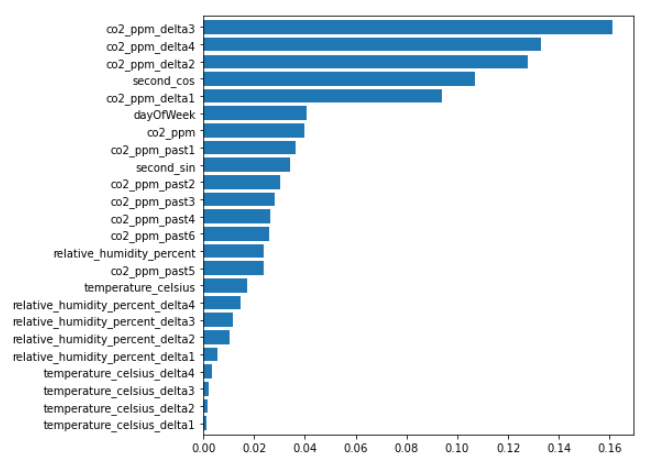
\includegraphics[width=0.8\textwidth]{pic/feature_importances.png}
    \caption{Feature Importances eines Random Forest}
    \label{fig:FI}
\end{figure}

In der o.g. Grafik sind neben den ursprünglichen Datenwerten nun auch Delta- und Shiftwerte zu sehen. Wie bereits 
im vorherigen Kapitel angedeutet, sieht man hier klar, dass die Temperatur- und Luftfeuchtigkeitswerte für 
die Errechnung der Labels kaum zu Rate gezogen werden. Weder die Grund- noch Deltawerte weisen eine hohe 
Wichtigkeit für das Model auf.
\newpage
Nach Exkludierung von Temperatur und Luftfeuchtigkeit wurden neue Deltas und Shifts für die CO2-Werte eingefügt 
und die Feature Importances erneut betrachtet. Es ist zu erkennen, dass auch die CO2-Werte von n Minuten zuvor 
ebenfalls nicht maßgeblich in die Berechnung einfließen.\\

\begin{figure}[h]
    \centering
    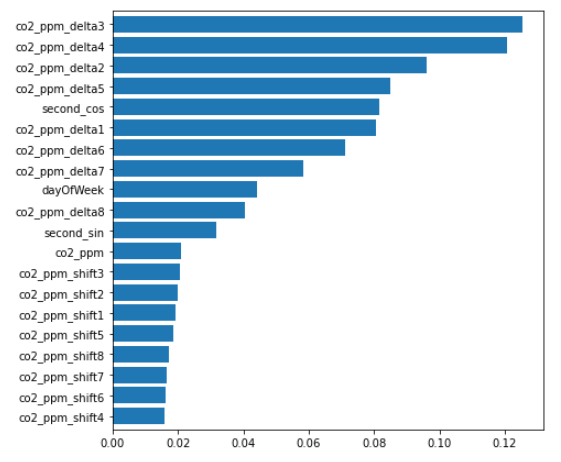
\includegraphics[width=0.8\textwidth]{pic/feature_importances_better.png}
    \caption{Feature Importances eines Random Forest}
    \label{fig:FIB}
\end{figure}

Der Graph bestätigt die Annahme, dass beim CO2 die Deltawerte deutlich ausschlaggebender sind, als die 
tatsächliche Messung zu einem bestimmten Moment. \\

Wenn diese Werte nur in solch geringem Maß zur Berechnung beitragen, muss ebenfalls die Schlussfolgerung daraus, 
dass die Genauigkeit auch ohne diese Werte innerhalb einer gewissen Toleranz konstant bleibt, überprüft werden.
\\
Im Folgenden werden beispielhaft vier verschiedene Feature Vektoren beschrieben, aus denen der Vektor, der im 
weiteren Verlauf des Projektes benutzt werden sollte, abgeleitet wurde.
\begin{center}
    \begin{tabular}{ |c||c| } 
     \hline
     Feature Vektor & Beschreibung \\ 
     \hline\hline
     FV1 & Temperatur und Luftfeuchtigkeit mit Shift-Werten\\ 
     FV2 & Temperatur und Luftfeuchtigkeit ohne Shift-Werte \\ 
     FV3 & Keine Temperatur- und Luftfeuchtigkeitswerte \\ 
     FV4 & FV3 ohne CO2-Shift-Werte \\
     \hline
    \end{tabular}
\end{center}

Mit diesen vier Vektoren wurden nun verschiedene Modelle trainiert und deren Genauigkeiten gegenübergestellt.

\begin{center}
    \begin{tabular}{|p{1.5cm}||p{2cm}| p{2cm}| p{2cm}| p{2cm}| p{2cm}|} 
        \hline
        Feature-Vektor&RF &SV &GB &KNN&LR \\ [0.5ex] 
        \hline\hline
        FV1&0.944805&	0.912594&	0.943618&	0.926824&   0.935428\\
        \hline
        FV2&0.946477&	0.918528&	0.931867&	0.925483&   0.916739\\
        \hline
        FV3&0.945256&	0.917241&	0.944554&	0.930148&   0.938136\\
        \hline
        FV4&0.945725&	0.912095&	0.947024&	0.929685&   0.931573\\
        \hline
    \end{tabular}\\        
\end{center}

\begin{figure}[h]
    \centering
    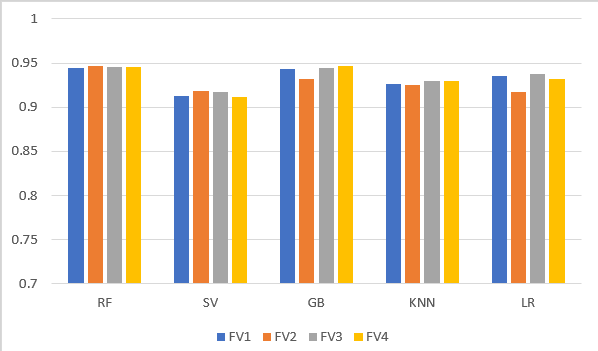
\includegraphics[width=0.8\textwidth]{pic/FV_comp.png}
    \caption{Vergleich der Genauigkeiten}
    \label{fig:FIB}
\end{figure}

Wie deutlich sichtbar ist, sind die Genauigkeiten fast identisch. Dies war Anlass sowohl die Temperatur- und 
Luftfeuchtigkeitswerte, als auch die Shift-Werte der CO2-Messungen nicht weiter zu betrachten.\\\\
\newpage
Aus diesen Betrachtungen ergab sich folgender FV der für den weiteren Verlauf des Projektes genutzt wurde:\\

\begin{center}
    \begin{tabular}{ |c||c| } 
     \hline
     Feld & Beschreibung \\ 
     \hline\hline
     second\_sin & timestamp-Sinusanteil\\
     second\_cos & timestamp-Cosinusanteil\\
     day\_of\_week & Wochentag der Messung\\
     co2\_ppm & CO2-Wert\\ 
     co2\_ppm\_delta1 & Delta zum CO2-Wert vor 2 Minuten\\ 
     co2\_ppm\_delta2 & Delta zum CO2-Wert vor 4 Minuten\\ 
     co2\_ppm\_delta3 & Delta zum CO2-Wert vor 6 Minuten\\ 
     co2\_ppm\_delta4 & Delta zum CO2-Wert vor 8 Minuten\\ 
     co2\_ppm\_delta5 & Delta zum CO2-Wert vor 10 Minuten\\ 
     co2\_ppm\_delta6 & Delta zum CO2-Wert vor 12 Minuten\\ 
     co2\_ppm\_delta7 & Delta zum CO2-Wert vor 14 Minuten\\ 
     co2\_ppm\_delta8 & Delta zum CO2-Wert vor 16 Minuten\\ 
     \hline
    \end{tabular}
\end{center}

\newpage
\section{Ergebnisse}
Da nicht alle Algorithmen auf die gleiche Weise evaluiert und grafisch dargestellt werden können, sollen 
die Ergebnisse zu 
\begin{itemize}
    \item Clustering Modellen
    \item Decision Tree Modellen
    \item Neuralen Netzwerken
\end{itemize}
einzeln betrachtet.

\subsection{Clustering Modelle}

\subsection{Decision Tree Modelle}
Die ausgewählten Algorithmen konnten mit dem ausgewählten FV bei der Erwartungsberechnung über das gesamte 
Datenset eine Genauigkeit von etwa 94\% erreichen. Eine \textit{Confusion Matrix}, welche die errechneten 
Werte den tatsächlichen gegenüberstellt, zeigt, dass im hier benutzten Beispiel, ein Random Forest Classifier 
selbst bei der starken Unausgeglichenheit des Datensets ähnlich viele Fehler in sowohl An- als auch Abwesenheit 
macht.

\begin{figure}[h]
    \centering
    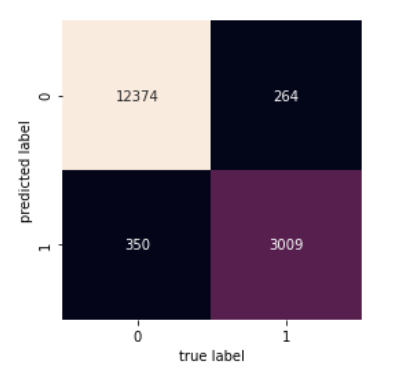
\includegraphics[width=0.5\textwidth]{pic/confusion_matrix.png}
    \caption{Confusion Matrix eines RFC}
    \label{fig:ConMatrix}
\end{figure}

In den Feldern oben links und unten rechts ist jeweils zu sehen, wann das Modell eine richtige Erwartung 
für jeweils Ab- und Anwesenheit errechnet hat, während die Felder oben rechts und unten links jeweils die falschen
Erwartung für beide Werte zeigen.\\\\

\newpage
Es ist ebenfalls aufschlussreich die erwarteten Labelwerte mit den tatsächlichen grafisch gegenüberzustellen, 
indem man das ursprüngliche Datenset mit timestamp und CO2-Wert zeichnet. Dabei wird die gemessene Anwesenheit 
farblich als gelb für an- und blau für abwesend eingefärbt.

\begin{figure}[h]
    \centering
    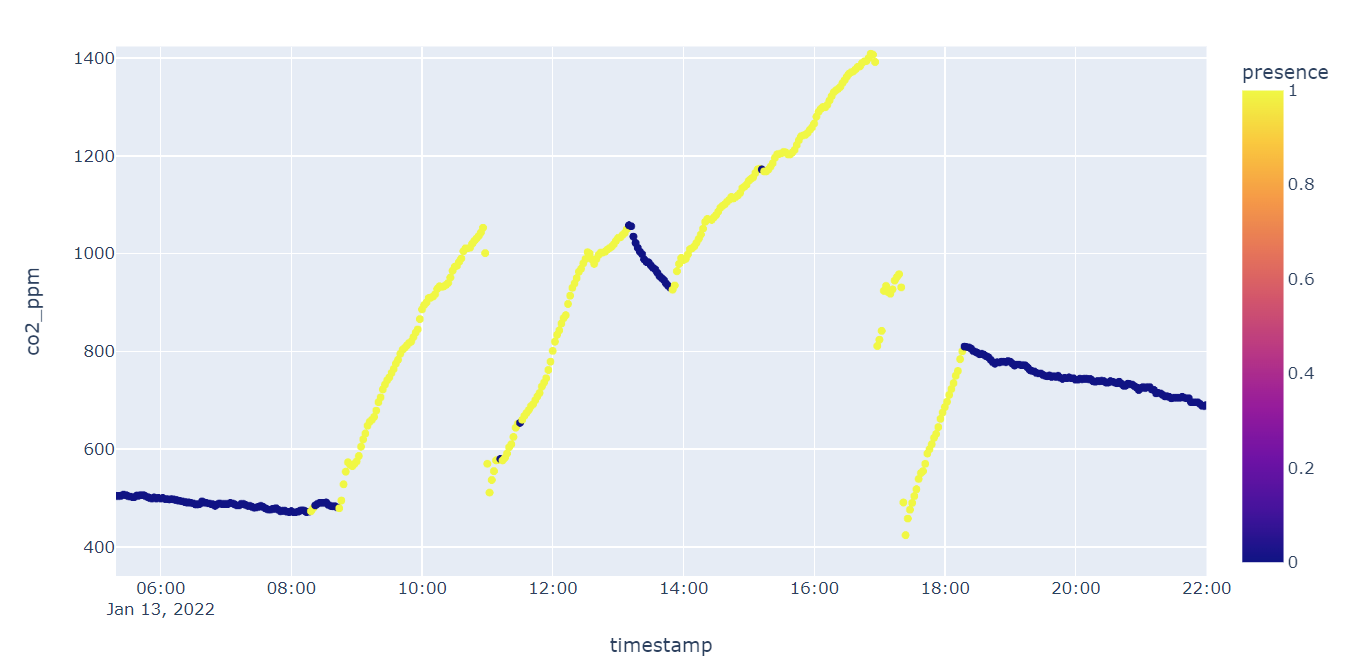
\includegraphics[width=0.9\textwidth]{pic/nov23_actual.png}
    \caption{Messwerte des 13. Januar}
    \label{fig:ConMatrix}
\end{figure}

Löscht man aus dieser Datenreihe die tatsächlichen Labelwerte und fügt stattdessen die errechneten 
Anwesenheitswerte des Modells ein, zeigt sich die hohe Genauigkeit deutlich. Bis auf einige kleine Fehler
trifft das Modell eine sehr präzise Aussage über die aktuelle Anwesenheit.

\begin{figure}[h]
    \centering
    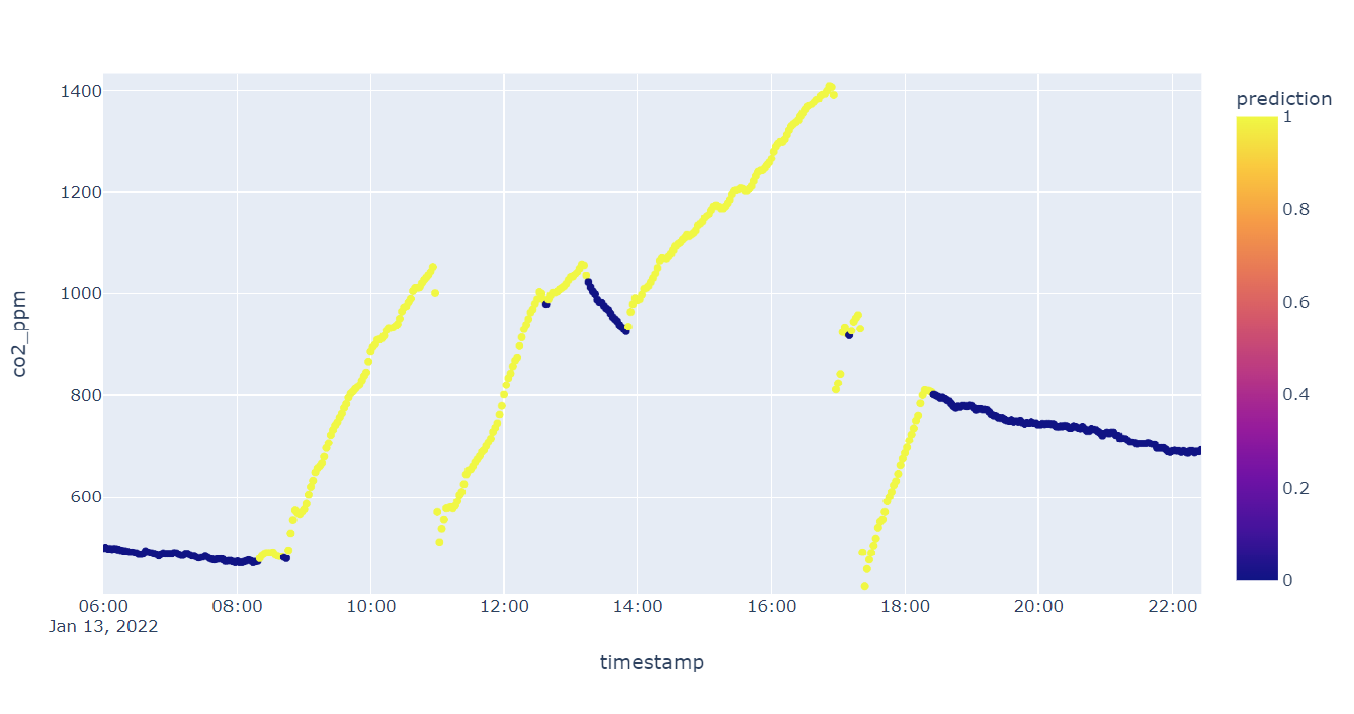
\includegraphics[width=0.9\textwidth]{pic/nov23_predicted.png}
    \caption{Messwerte des 13. Januar}
    \label{fig:ConMatrix}
\end{figure}

Dieses Ergebnis konnte über eine Vielzahl von Kombinationen verschiedener Räume und Modelle weiterhin
bestätigt und repliziert werden. Die Tatsache, dass die Genauigkeiten aller Modelle so nah beieinander 
liegen, rührt daher, dass dieses Datenset ein typisches Klassifizierungsproblem darstellt,
wodurch die sich wiederholenden Schemata in den CO2-Werten von einer Vielzahl von Algorithmen schnell 
erkannt und verarbeitet werden können.

Beim Tuning der ausgewählten Modelle wurden als Parameter-Optionen ausschließlich Werte gewählt, die nicht 
den Standardwerten der Modelle entsprechen. Somit sollte das GridSearchCV-Modul ausschließlich in der Menge 
von Parametern nach möglichen suchen, die nicht den Standard-Einstellungen entsprechen.

\begin{figure}[h]
    \centering
    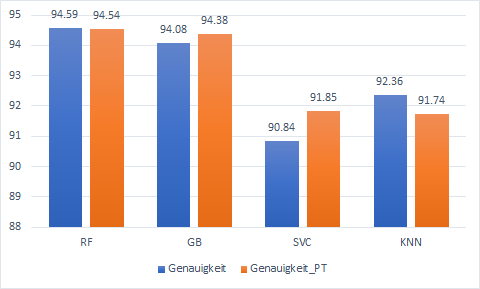
\includegraphics[width=0.7\textwidth]{pic/param_eval.png}
    \caption{Ergebnisse des Parameter Tuning}
    \label{fig:PT_eval}
\end{figure}

Es ist zu sehen, dass das Parameter Tuning die Genauigkeit der Modelle im erwarteten Rahmen erhöht oder 
verringert hat. Dies bestätigt die Annahme, dass dieser Anwendungsfall ein typisches Klassifizierungsproblem 
darstellt, weshalb die Modelle nicht mehr maßgeblich verbessert werden können. Der Schritt des Parameter Tunings 
sollte trotzdem grundsätzlich immer durchgeführt werden, um zu erkennen, ob man durch eine einfache Änderung 
der Parameter eine Verbesserung des Modells hervorbringen kann.\\

Zusätzlich wurden die \textit{ROC-Curves} der True- und False-Positives gegeneinander gezeichent um zu erknennen 
inwiefern die Ergebnisse zufällig oder errechnet sind.

\begin{figure}[h]
    \centering
    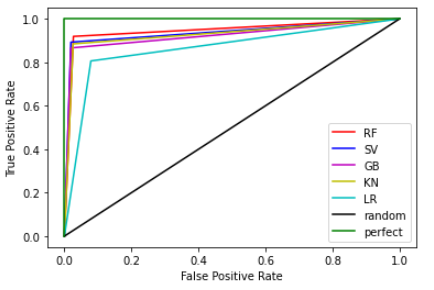
\includegraphics[width=0.7\textwidth]{pic/roc_curves.png}
    \caption{ROC-Curves aller Modelle}
    \label{fig:PT_eval}
\end{figure}

Man sieht deutlich, wie alle Modelle sehr ähnliche Ergebnisse aufweisen. Keines der Modelle weist anzeichen 
auf, dass Ergebnisse wegen mangelnder Informationen erraten werden.

\subsection{Neurale Netzwerke}
Die beiden implementierten Neuronalen Netze konnten eine ähnliche Leistung, wie die bereits oben genannten 
Algorithmen erzielen. Beide Modelle wurden über so viele Iterationen (Epochen) trainiert, bis ersichtlich war,
dass die Genauigkeit gegen einen Wert konvergiert. Zur Auswertung wurden hier die \textit{Accuracy-} und 
\textit{Loss}-Funktionen genutzt. Die Genauigkeit beschreibt, wie bei den anderen Modellen das Verhältnis
zwischen richtigen und falschen Berechnungen.\\
Die Loss-Funktion hingegen gibt die Abweichung einer Schätzung zum tatsächlichen Wert an. Diese beiden Wert 
werden nach jeder Epoche ausgewertet, während zunächst der Erfolg während des Trainigs als \textit{train}
angegeben wird und danach das Modell an einem zufälligen Teil des Validierungssets \textit{val} getestet wird.
Liegen diese beiden Kurven nah beieinander, ist dies ein gutes Anzeichen für ein funktionierndes Modell ohne 
Over- oder Underfitting, da sowohl beim Training als auch bei der Validierung die Genauigkeiten Ähnlichkeiten
aufweisen, während zugleich die Loss-Funktion minimiert wird.

\begin{figure}[h]
    \centering
    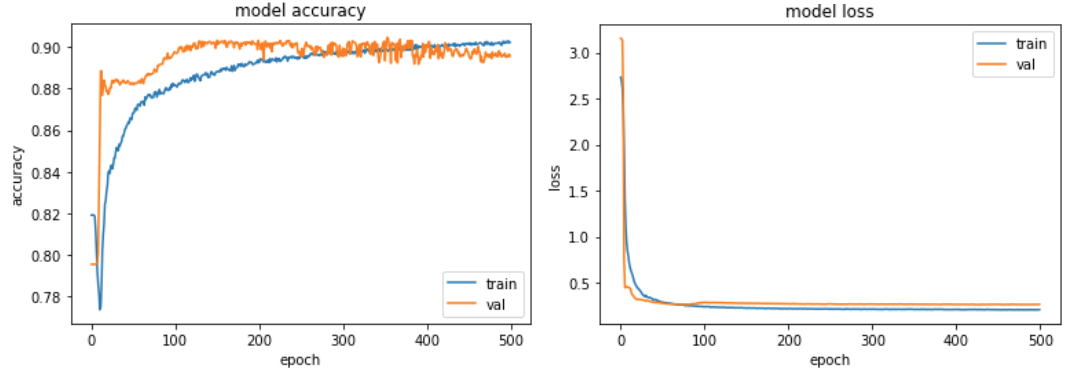
\includegraphics[width=0.9\textwidth]{pic/eval_NN.png}
    \caption{Ergebnisse des NN}
    \label{fig:PT_eval}
\end{figure}

\begin{figure}[h]
    \centering
    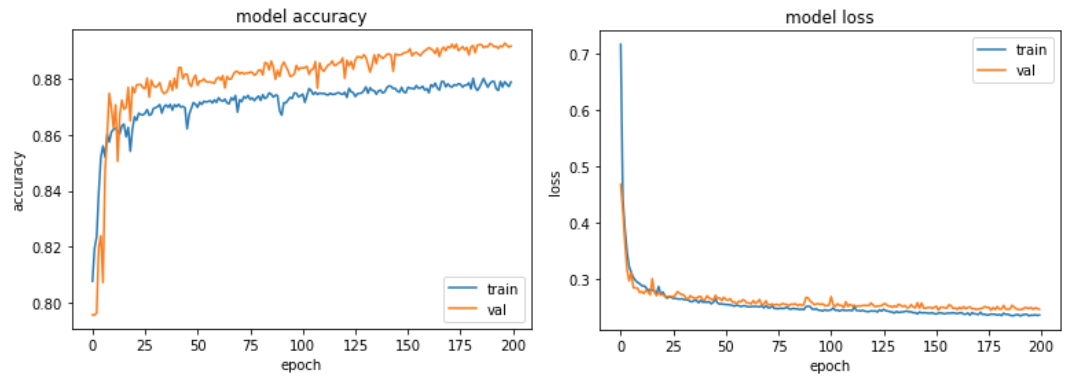
\includegraphics[width=0.9\textwidth]{pic/eval_LSTM.png}
    \caption{Ergebnisse des LSTM}
    \label{fig:PT_eval}
\end{figure}

Wie zu sehen ist, weisen beide Arten neuraler Netzwerke diese Eigenschaften auf. Die Genauigkeiten beider Modelle
konvergierten auch nach verschiedenen Epochen-Werten etwa bei 89\%.